\section{Results}

%\begin{figure}[h]
%	\centering
%	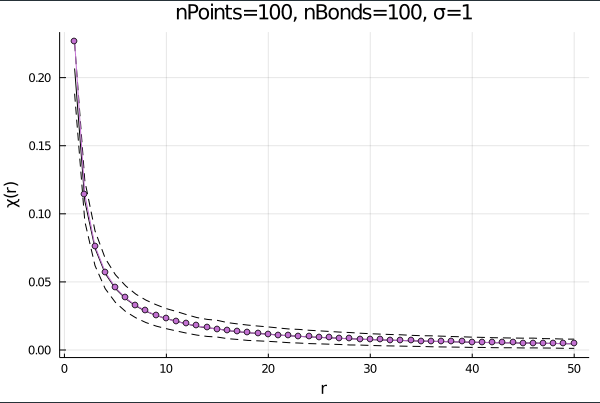
\includegraphics[width=0.8\textwidth]{figures/correlationFunction.png}
%	\caption{The average correlation function (black) $\xi(r)$ and its standard deviation (dashed lines) of  1000 realizations of a connectivity graph with $N=100, nBonds=100, \sigma=1$. In pink, dotted, the fit of the average correlation function to the curve $y = (4.5 r + 0.5) ^ {-1} $.} 
%	\label{fig:correlationFunction}
%\end{figure}
%
% Figure \ref{fig:nClusters} shows the mean number of clusters and the variation of the mean as a function of $N_l$, for different $\sigma$, as indicated in the legend. The normalized size distribution of the clusters is reported in Figure \ref{fig:clusterLengthDistribution}.
%
%With a given probability of forming a bond between two nodes that are at a distance $r$ away from each other to be $r^{-\sigma}$, we expect the correlation function $\xi(r)$ (i.e. the distribution of distances at which two nodes are bound) to follow $\sim r^{-\sigma}$. We show in the figure \ref{fig:correlationFunction} the measured average (black, solid line) correlation function and its standard deviation (black, dashed lines) after generating 1000 realizations of the connection graph using Walker's Alias algorithm to draw the bonds among the nodes. In pink, overlayed on top of the black curve, the fit of the average $\xi(r)$ is shown. We fit $\xi(r)$ to the curve $y = (a r + b) ^{-\sigma}$ and obtain a perfect overlay between the data (the average $\xi(r)$) and the fit curve.
%


Figure \ref{fig:nClusters} displays the change in number of clusters for different configurations, for a constant $N$, as a function of the number of bonds $N_l.$ Different curves correspond to different  $\sigma$, as indicated by the legend. The standard deviation of the sample mean is reported.

Figure \ref{fig:clusterLengthDistribution} displays the size distribution of the clusters for different $N_l$, for fixed $N.$ The three panels display the distributions for different values of  $\sigma.$ For visualization purposes, the curves are normalised, since there are less available clusters of length  $N$,  than there are clusters of length 1 (isolated sites), which leading to underrepresentation.

The order parameter of choice is the magnetization $m = \frac{1}{N}\sum_i s_i $ of the spin chain. Figure \ref{fig:magnetization} shows the magnetization of the spin chain, as the Metropolis algorithm advances, with $N = N_l = 4096, \sigma = 0.5$. The top panel shows the magnetization for 50 different starting spin seeds, and the bottom panel presents the averaging of $^2$ across said spin seeds in blue. The curve  $y = 10^{-5.5} x^{1.7} $ is given in red, for reference.

\begin{figure}
	\centering
	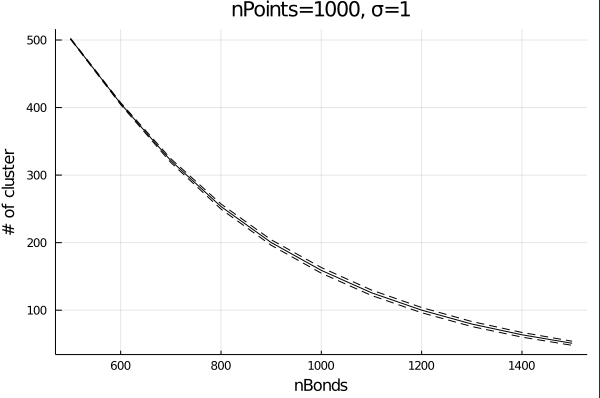
\includegraphics[width=0.8\textwidth]{figures/nClusters.pdf}
	\caption{Average number of clusters and variation of the mean as a function of number of bonds, for $N=50$ and varying $\sigma$, as indicated by the legend.}
	\label{fig:nClusters}
\end{figure}

\begin{figure}
		\centering
		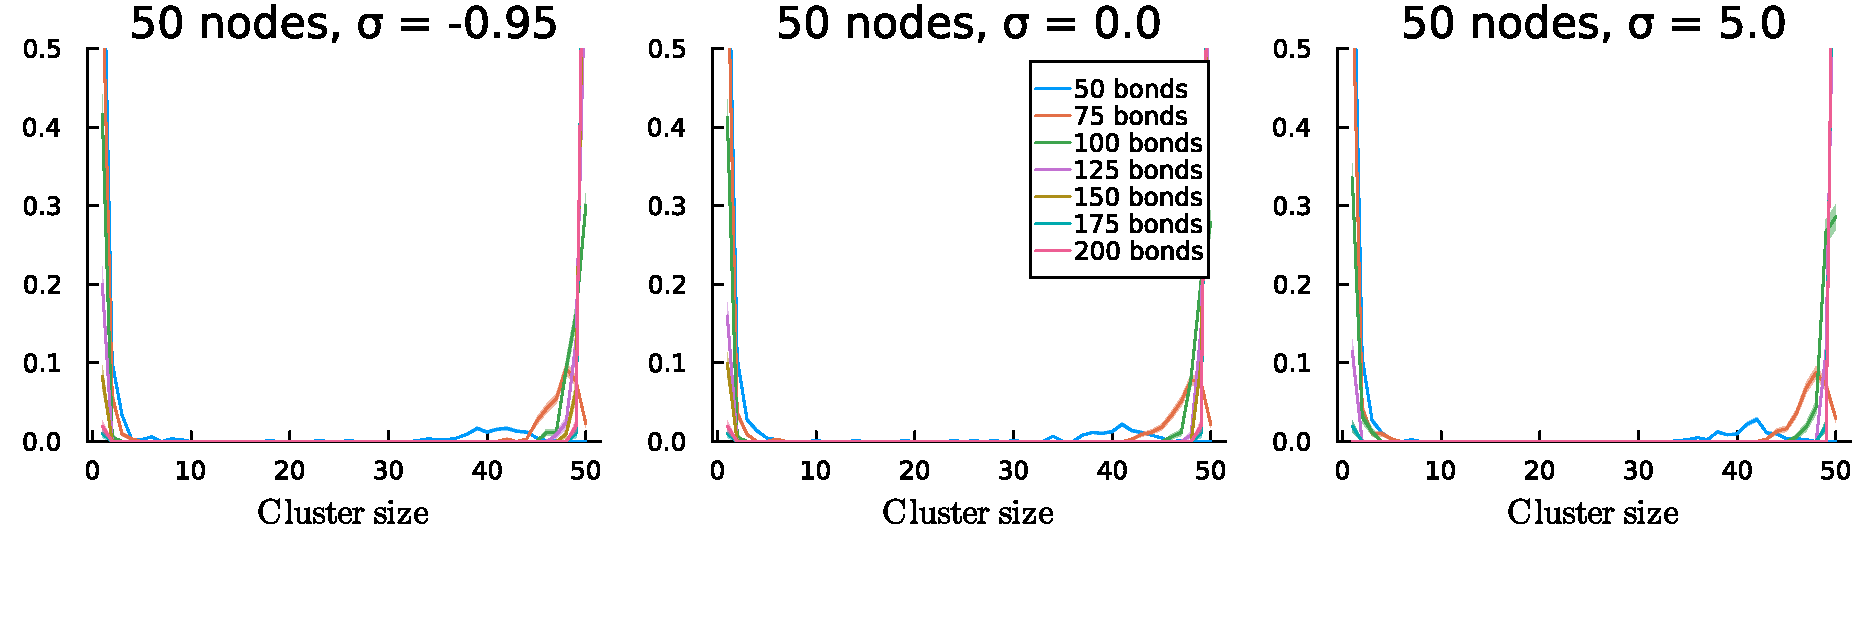
\includegraphics[width=\textwidth]{figures/clusterSizeDistribution.pdf}
	\caption{Normalized distributions of cluster sizes for fixed number of nodes $N=100$ and  varying $\sigma$ values, as indicated at the top of each panel, for different number of bonds among the nodes, as indicated in the legend of the middle panel.}
	\label{fig:clusterLengthDistribution}
\end{figure}
\begin{figure}[p]
	\centering
	\begin{subfigure}{0.8\textwidth}
	\includegraphics[width=1\textwidth]{figures/isingRuns/T_0.1_nPoints_4096_nBonds_4096_sigma_0.2.pdf}
	\end{subfigure}
	\begin{subfigure}{0.8\textwidth}
	\includegraphics[width=1\textwidth]{figures/m2Runs/T_0.1_nPoints_4096_nBonds_4096_sigma_0.2.pdf}
	\end{subfigure}
	\caption{ Magnetization $m$ of the 1-dimensional spin chain with periodic boundary conditions, as iterations of the Metropolis advance, for different spin seeds and the same $J_{ij}$. In the top panel, the magnetization of the spin chain for different starting seeds and different connectivities $J_{ij}$. In the bottom panel, the magnetization squared, averaged across runs. The curve $y=10^{-5.5} x^{1.7}$ is shown in red, for reference. Calculations here are done with $N = N_l = 4096, \sigma = 0.5.$}
	\label{fig:magnetization}
\end{figure}
